\documentclass[hyperref]{beamer}
\usepackage{beamerthemesplit}
\usepackage{graphicx}
\usepackage{mathptmx}           % replacement for obsolete \usepackage{times}
\usepackage[scaled=.90]{helvet} % replacement for obsolete \usepackage{times}
\usepackage{courier}            % replacement for obsolete \usepackage{times}

\usepackage{tikz}
\usetikzlibrary{shapes.arrows,chains,positioning,automata,trees,calc}
\usetikzlibrary{patterns}
\usetikzlibrary{decorations.pathmorphing,decorations.markings}
\usepackage{times,latexsym,amsfonts,amssymb,amsmath,graphicx,url,bbm,rotating,siunitx}
\usepackage{multirow,hhline,arydshln,array,color,stmaryrd}
\definecolor{darkred}{rgb}{0.5, 0.0, 0.0}
\definecolor{darkgreen}{rgb}{0.0, 0.4, 0.0}
\definecolor{darkblue}{rgb}{0.0, 0.0, 0.5}

% set up Beamer style with Stanford colors and logo
% logo is available at http://nlp.stanford.edu/local/nlp-logos/nlp-logo.pdf
\useinnertheme{rounded}
\useoutertheme{infolines}
\usecolortheme{beaver}
\setbeamercolor{block title}{fg=white,bg=darkred!75!black}
\setbeamercolor{block body}{parent=normal text,bg=black!5!bg}
\setbeamercolor{item projected}{bg=darkred}
\logo{
\includegraphics[height=1cm]{../img/nlp-logo.pdf}}

% title page information
\title{NaturalLI: Natural Logic for Common Sense Reasoning}
\subtitle{}
\author{Gabor Angeli, Chris Manning}
\date{June 13, 2014}
\institute[Stanford]{Stanford University}

\input ../macros.tex
\input ../figures.tex

\begin{document}
\begin{frame}
  \titlepage
\end{frame}

%%%%%%%%%%%%%%%%%%% 
% COMMON SENSE REASONING
%%%%%%%%%%%%%%%%%%%
\begin{frame}{Common Sense Reasoning}
\begin{tabular}{cc}
  \green{Cats play with yarn} & \red{Cats play with computers} \\
  \vspace{0.25cm} \\
  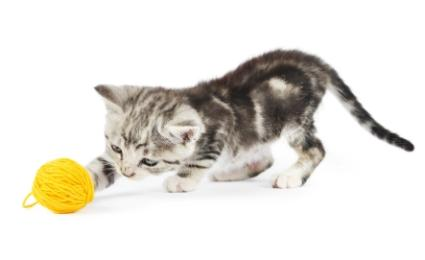
\includegraphics[width=5cm]{../img/yarn-cat.jpg} & \pause 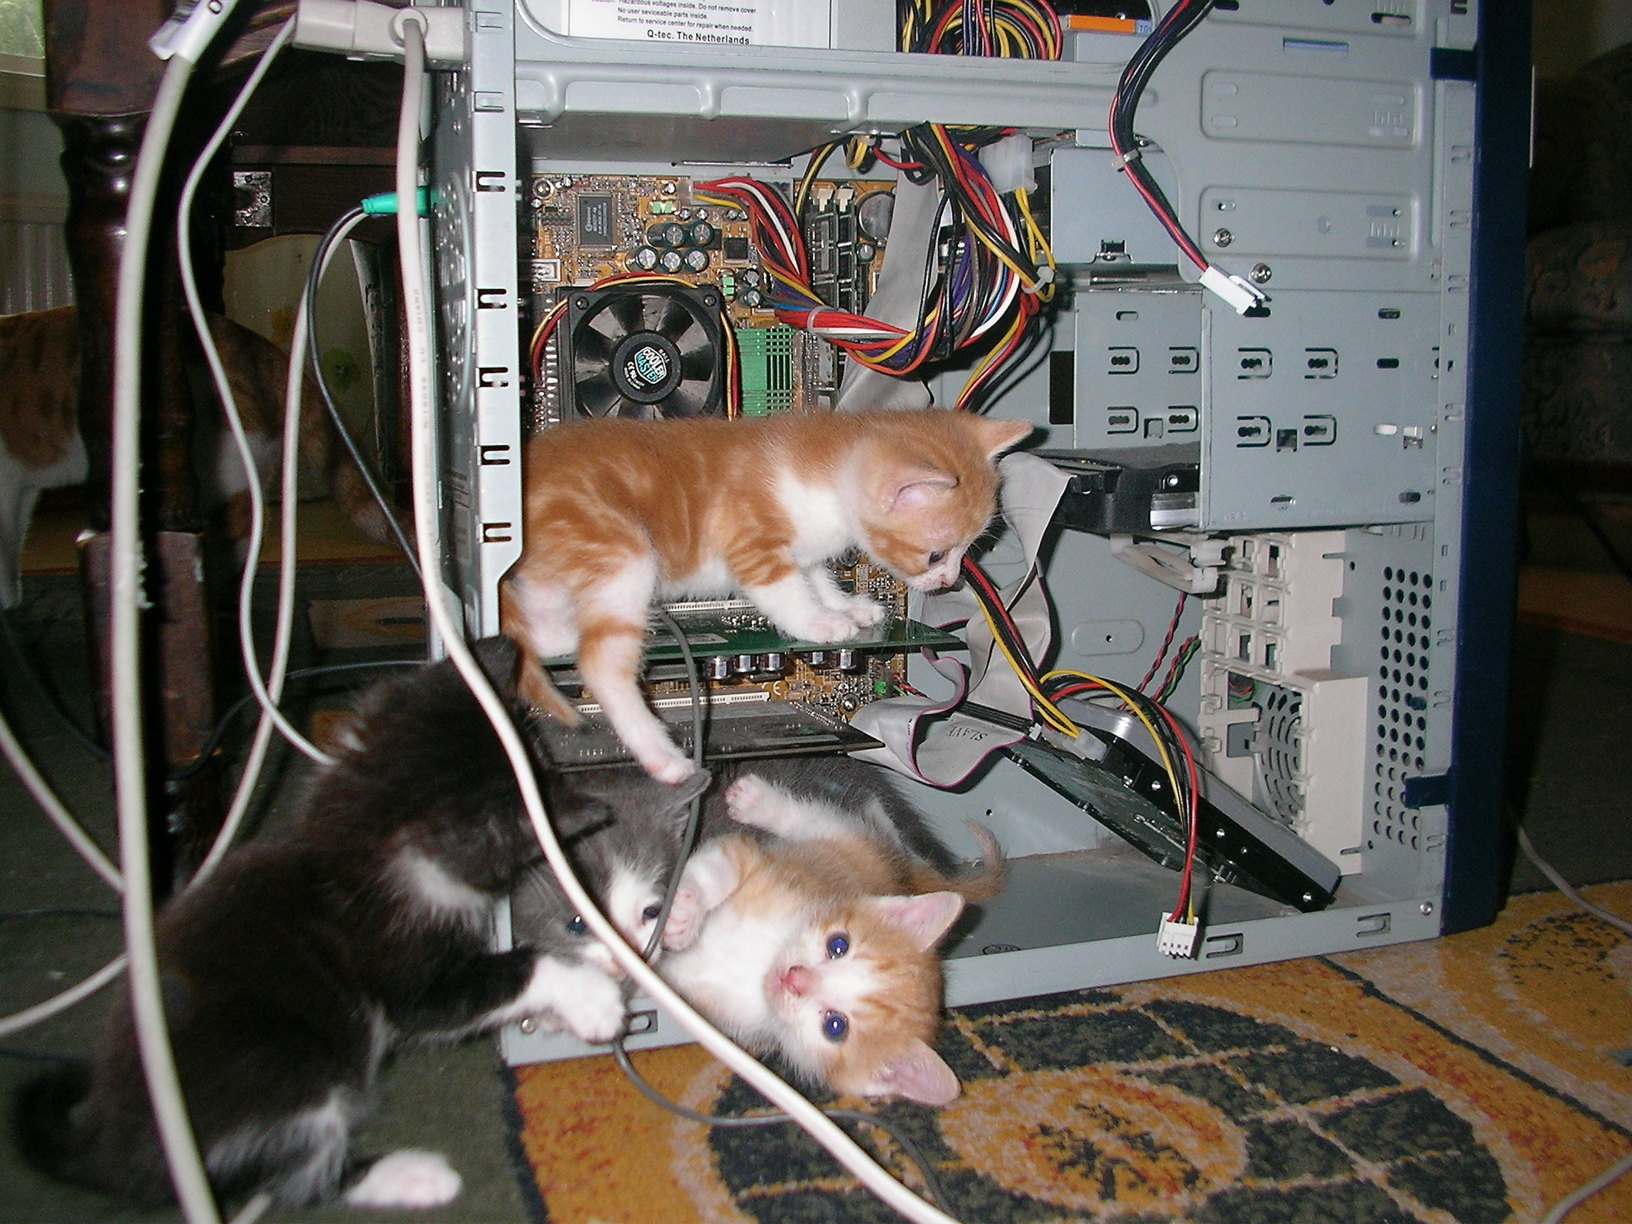
\includegraphics[width=5cm]{../img/computer-cat.jpg}
\end{tabular}
\end{frame}

%%%%%%%%%%%%%%%%%%% 
% COMMON SENSE REASONING 2
%%%%%%%%%%%%%%%%%%%
\begin{frame}{Common Sense Reasoning for Vision}
\begin{tabular}{cc}
  \red{Dogs drive cars} & \green{People drive cars} \\
  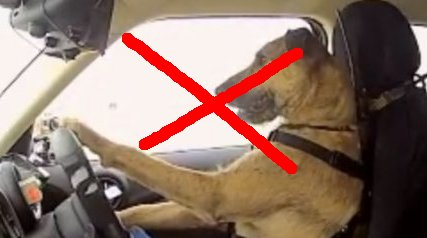
\includegraphics[height=3cm]{../img/dog-driving.jpg} & 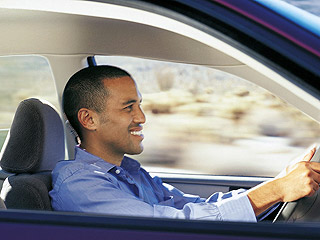
\includegraphics[height=3cm]{../img/person-driving.jpg}  \\
  \vspace{0.25cm} \\
  \pause \red{Baseball is played underwater} & \green{Baseball is played on grass} \\
  
\includegraphics[height=3cm]{../img/baseball-underwater.jpg} & 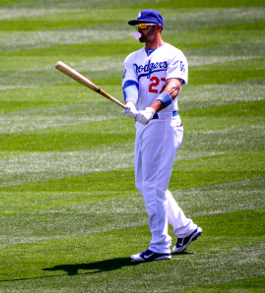
\includegraphics[height=3cm]{../img/baseball-grass.jpg} \\
\end{tabular}
\end{frame}

%%%%%%%%%%%%%%%%%%% 
% NATLOG AS SYLLOGISM
%%%%%%%%%%%%%%%%%%%
\begin{frame}{Natural Logic}
\begin{center}
\w{A cat ate a mouse} $\xRightarrow{?}$ \w{No carnivores eat animals}
\end{center}

\hh{First-Order Logic} \\
\hspace{0.5cm} \h{Start with text:} \w{A cat ate a mouse} \\
\pause
\hspace{0.5cm} \h{Translate to symbols:} $\exists c \exists m ~~\left( \textrm{cat}(c) \land \textrm{mouse}(m) \land \textrm{eat}(c,m) \right)$ \\
\pause
\hspace{0.5cm} \h{Run inference:} $\dots$ \\
\pause
\hspace{0.5cm} \h{Get Answer:} $\exists v ~~ \textrm{carnivore}(v) \rightarrow \left( \exists a ~~ \textrm{animal}(a) \land \textrm{eat}(v, a) \right) ~~~~~ \bot$
\vspace{0.5cm}
\pause

\hh{Natural Logic} is a logic whose syntax is natural language. \\
\vspace{0.5cm}
\pause

\hh{Think Syllogisms}:\\
\hspace{0.5cm} \textcolor<7->[rgb]{0,0.5,0}{All Greeks are men.} \\
\hspace{0.5cm} All \textbf<8->{men} are mortal. \\
\hspace{0.5cm} All \textbf<8->{Greeks} are mortal. \\
\end{frame}

%%%%%%%%%%%%%%%%%%% 
% NATURALLI SEARCH
%%%%%%%%%%%%%%%%%%%
\begin{frame}{Natural Logic for Knowledge Base Completion}
\begin{tabular}{ll}
  \h{Input:} & A query fact and a corpus of text snippets \\
  \h{Output:} & The truth of the query
\end{tabular}
\vspace{0.25cm}
\pause

\hh{Search over mutations from query:}
\begin{center}
  \resizebox{8cm}{!}{\teaserSearch}
\end{center}
\end{frame}

%%%%%%%%%%%%%%%%%%% 
% NATURALLI SEARCH
%%%%%%%%%%%%%%%%%%%
\begin{frame}{Natural Logic for Knowledge Base Completion}
\begin{center}
  \resizebox{5cm}{!}{\teaserSearch}
\end{center}

\hh{Each mutation has a cost $c$}
\begin{itemize}
  \item \h{Low cost:} \w{some cats have tails} $\Rightarrow$ \w{some felines have tails}
  \item \h{High cost:} \w{some cats have tails} $\Rightarrow$ \w{some dogs have tails}
\end{itemize}
\pause

\hh{Costs are negative weights}
\begin{itemize}
  \item $P(true) = \frac{1}{2} + \frac{1}{1 + e^{c \cdot f(\textrm{path})}}$
\end{itemize}
\pause

\hh{Search gets better as we learn}
\end{frame}


%%%%%%%%%%%%%%%%%%% 
% NATURALLI SEARCH
%%%%%%%%%%%%%%%%%%%
\begin{frame}{Looking for Applications!}
\begin{center}
  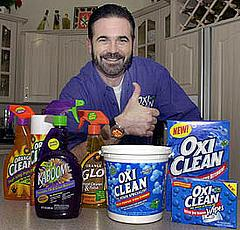
\includegraphics[width=3cm]{../img/billy-mays.jpg}
\end{center}
\pause

\hh{Strictly better than querying a knowledge base}
\begin{itemize}
  \item 12\% recall $\rightarrow$ 48\% recall @ 93\% precision
\end{itemize}
\pause

\hh{Strictly better fuzzy queries}
\begin{itemize}
  \item Checks logical entailment, not just \textit{fuzziness}
  \item Support doesn't have to be lexically similar
\end{itemize}
\pause

\hh{Sometimes even a bit clever}
\end{frame}

%%%%%%%%%%%%%%%%%%% 
% THANKS
%%%%%%%%%%%%%%%%%%%
\begin{frame}{}
\begin{center}
  \hh{\huge{Thanks!}} \\
  \vspace{1cm}
  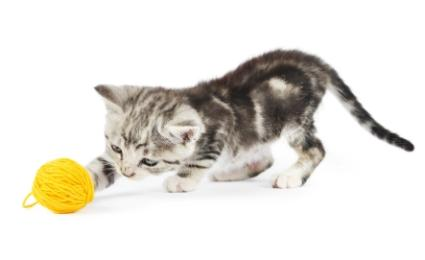
\includegraphics[width=3cm]{../img/yarn-cat.jpg}
\end{center}
\end{frame}



%%%%%%%%%%%%%%%%%%%% 
%% NATURAL LOGIC AS MONOTONICITY
%%%%%%%%%%%%%%%%%%%%
%\begin{frame}{Natural Logic and Monotonicity}
%\pause
%\hh{Mathematical Syntax Analogy:}
%\begin{itemize}
%  \item $2 \le 3$
%  \item $f(x) = e^x$ is monotone (i.e., non-decreasing).
%  \item $g(x) = -x$ is antitone (i.e., non-increasing).
%  \pause
%  \item \h{Query:} Is $e^{-3} \le e^{-2}$?
%  \pause
%  \begin{tabular}{ll}
%    Option 1: & $0.05 \le 0.14$, therefore $e^{-3} \le e^{-2}$. \\
%    \pause
%    Natural Logic: & $2 \le 3 \hspace{0.25cm} \Rightarrow \hspace{0.25cm}  e^2 \le e^3 \hspace{0.25cm} \Rightarrow \hspace{0.25cm} e^{-\textbf<6->{3}} \leq e^{-\textbf<6->{2}}$.
%    \pause % for bolding
%  \end{tabular}
%\end{itemize}
%\vspace{0.1cm}
%\pause
%
%\hh{Language Equivalent}
%\begin{itemize}
%  \item $\denote{cats} \subseteq \denote{felines}$ \pause (\w{all cats are felines}).
%  \pause
%  \item $f(x) = ``\textit{some } x$'' is monotone.
%  \item $g(x) = ``\textit{no dogs chase } x$'' is antitone.
%  \pause
%  \item \h{Query:} \textit{no dogs chase some \textbf<11->{felines}} $\xRightarrow{?}$ \textit{no dogs chase some \textbf<11->{cats}}
%\end{itemize}
%\end{frame}

\end{document}
